\section{Statistical Testing Procedure}

\begin{frame}
  \begin{center}
    {\bf Part II -- General Procedure of Statistical Testing}
  \end{center}
\end{frame}

\subsection{Ideas}
\begin{frame}{Outline of the Procedure for the NHST}
  The objective of the statistical test is to answer the question:\\
  "Do we have enough evidence to prefer the Alternate Hypothesis to the Null Hypothesis"?\bigskip

  In other words, $P(x|H_0)$ low enough that we need to {\bf reject} the null hypothesis?\bigskip

  To make this decision, we calculate an {\bf estimate} for the parameter of interest (x) in the hypothesis, and compare this value with a {\bf Expected/Rejection Region}.
  \begin{center}
    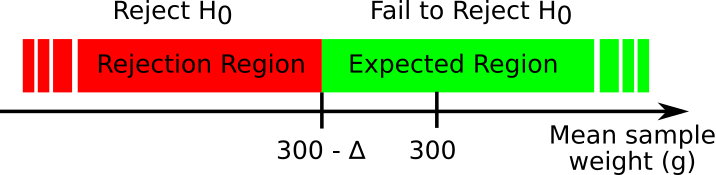
\includegraphics[width=.8\textwidth]{../img/critical_region}
  \end{center}
\end{frame}

\begin{frame}{Outline of the Procedure for the NHST}{Inference Errors}
  There are four possible results to a Statistical Inference Test:
  \begin{itemize}
    \item The estimate falls in the expected region: We can't reject the Null Hypothesis.
    \item The estimate falls in the reject region: We reject the Null Hypothesis.
    \item (Type I error): Estimate falls in the rejection region, but the Null Hypothesis is correct.
    \item (Type II error): Estimate falls in the expected region, but the Null Hypothesis is incorrect.
  \end{itemize}

  \begin{center}
    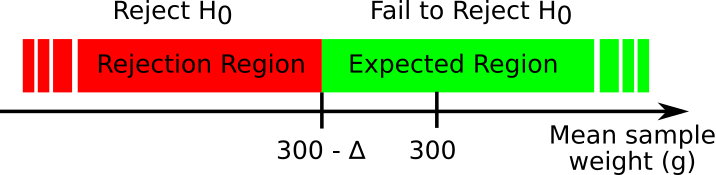
\includegraphics[width=.5\textwidth]{../img/critical_region}
  \end{center}

  These errors can happen because of large errors in the estimate, and/or because of error in the calculation of the expected region. By selecting good experiment parameters, we can control these errors to a degree.

\end{frame}

\subsection{Two Types of Errors}

\begin{frame}[t]{Type I Error (False Positive)}
{The data reject the $H_0$, when $H_0$ is true.}

  The probability of occurrence of a false positive in any hypothesis testing procedure is generally known as the \structure{significance level} ($\alpha$, or "alpha") of the test.\bigskip
    \begin{itemize}
      \item Significance Level $\alpha = P(\text{type I error}) = P(\text{reject }H_0|H_0\text{ is true})$
    \end{itemize}\vfill

  It is also called the \structure{confidence level} of a test, given by $(1-\alpha)$ or $100(1-\alpha)$\%\bigskip

  \begin{itemize}
    \item Confidence Level $100*(1-\alpha)$\%
  \end{itemize}
\end{frame}

\begin{frame}{Type I Error (False Positive)}{Controlling the probability of Type I Error by choosing $\alpha$}

  For a given statistical model, $H_0$, and sample, the probability of a type I error ($\alpha$) is the area of the sample distribution that falls under the threshold value.\medskip

  So, by selecting the threshold value, we can control $\alpha$.\bigskip

  \begin{columns}[T]
    \column{0.5\textwidth}
    In our example, \structure{assuming the package follows a normal distribution},
    we expect the sample mean to be $\mu$ with standard error $(\sigma / \sqrt{n})$.\bigskip

    We can calculate $\Delta$ so that the probability of
    the sample mean falling in the rejection region is $\alpha$

    % For a given sample, the value selected for $\alpha$ defines the threshold for the rejection of $H_0$. If $H_0$ is true (i.e., $\mu = 300$g), we can expect that the distribution of mean estimates is approximately normal
    % %\footnote{Assuming the CLT conditions are met},
    % with average 300g and standard error $(\sigma/\sqrt{n})$.
    %
    % To control the probability of Type I error (e.g. $\alpha=0.05$), we select the critical region so that the cumulative probability under the distribution of $\hat{x}$ inside that region is $1-\alpha=0.95$.
    \column{0.5\textwidth}
    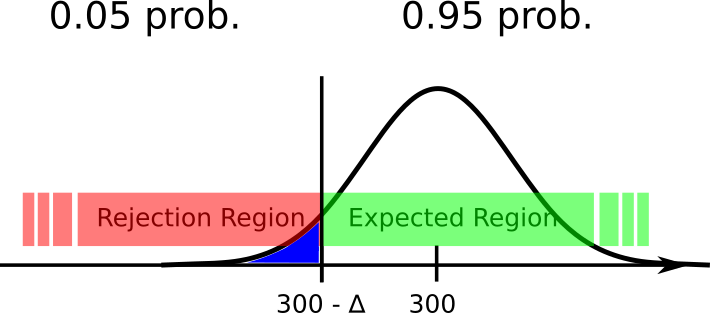
\includegraphics[width=\textwidth]{../img/critical_region_alpha}
  \end{columns}
\end{frame}

\begin{frame}{Type II Error (False Negative)}{The data does not reject $H_0$ when $H_0$ is false}
  The probability of occurrence of a false negative in any hypothesis testing procedure is generally represented by the Greek letter $\beta$:
  \begin{equation*}
    \beta = P(\text{type II error}) = P(\text{not reject }H_0|H_0\text{ is false})
  \end{equation*}\bigskip

  The quantity $(1 - \beta)$ is known as the {\bf power of the test}. It quantifies the test's sensitivity to effects that violate the null hypothesis.
\end{frame}

\begin{frame}{Type II Error (False Negative)}{Statistical Interpretation}
  \begin{columns}[T]
    \column{.7\textwidth}
    The probability of Type II error is harder to estimate precisely than the
    Type I error.\bigskip

    This is because it depends on \structure{the True Value of the parameter}.
    But this value {\bf is unknown when $H_0$ is false.}\bigskip

    The probability of Type II error is calculated as the area of the \structure{sampling region under the real parameter value} that falls in the \structure{acceptance region}.

    \column{.3\textwidth}
    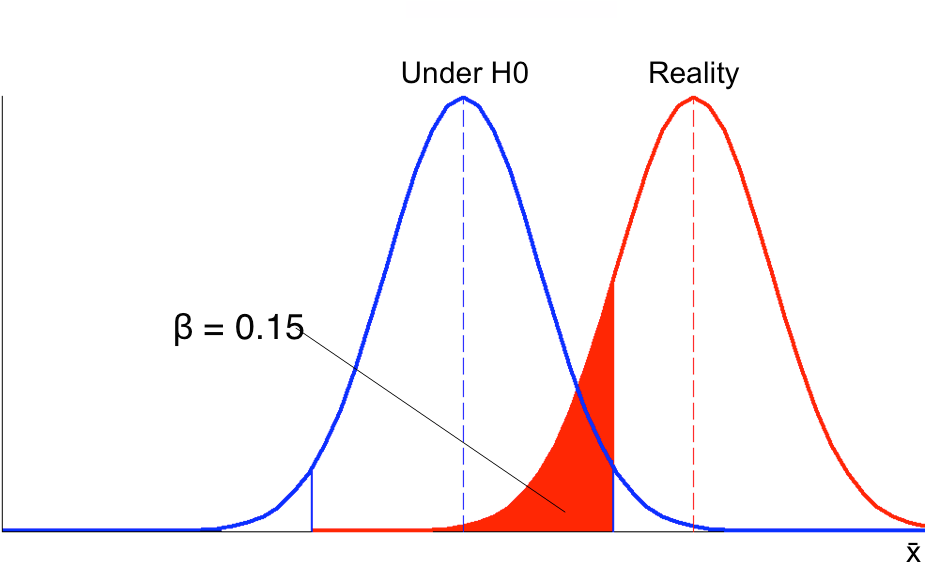
\includegraphics[width=\textwidth]{../img/beta-a}\\
    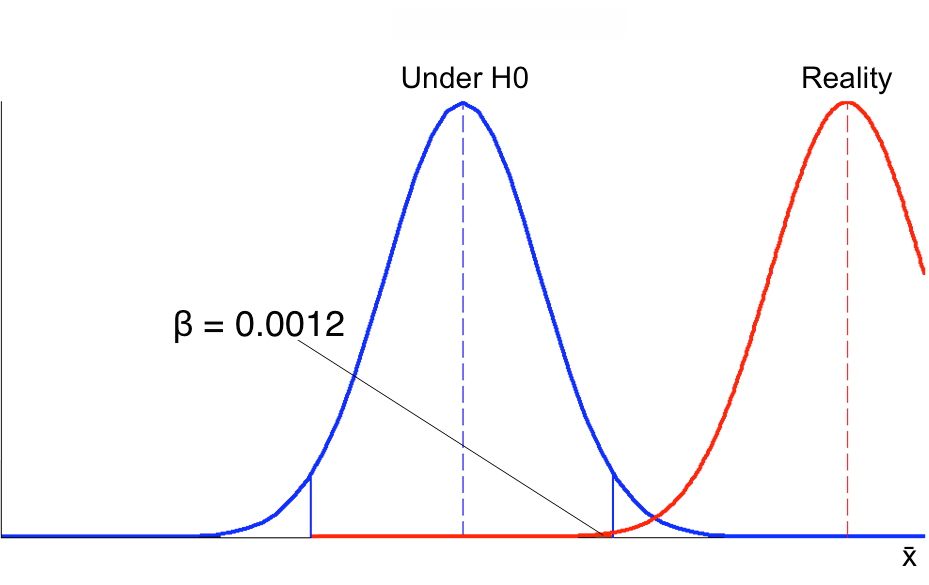
\includegraphics[width=\textwidth]{../img/beta-d}
  \end{columns}
\end{frame}

\begin{frame}{Type II Error (False Negative)}{Controlling the value of $\beta$}
  The power $\beta$ of a test is governed by several factors:
  \begin{itemize}
    \item {\bf Controllable factors}: significance level $\alpha$, size of the sample;
    \item {\bf Uncontrollable factors}: real value of the parameter, variance of the data;
  \end{itemize}\bigskip

  In general, it is possible to estimate the power of a test for \structure{a target desired difference} $|H_0 - H_1|$.\bigskip

  The interpretation of this calculation is "If the difference between the real value and $H_0$ is at least $|H_0 - H_1|$, the probability of a type II error is $\beta$"
\end{frame}

\begin{frame}{Considerations on Inference Errors}

  {\bf Type I Error $(\alpha)$ -- significance}: depends only on the distribution of the null hypothesis -- easier to control;
  \medskip

  {\bf Type II Error $(\beta)$ -- power}: depends on the real value of the parameter -- more difficult to specify and control;
  \bigskip

The two conclusions of a test of hypothesis are normally considered as follows:
  \begin{exampleblock}{}
    \begin{itemize}
      \item Rejection of $H_0$ (easy to control the error) - strong conclusion;
      \item Failure to Reject $H_0$ (hard to control the error) - weak conclusion;
    \end{itemize}
  \end{exampleblock}
  \alert{It is important to remember that failing to reject $H_0$ does not mean that there is evidence in favor of $H_0$!} -- it only suggests that $H_1$ is not better than the normal assumptions ($H_0$).
\end{frame}

\subsection{Calculating Examples}
\begin{frame}{Hypothesis testing}{General Procedure}
  \begin{enumerate}
    \item Identify the parameter of interest;
    \item Define $H_0$ and $H_1$ (also define if the test is one-sided or two-sided);
    \item Determined desired values for $\alpha$ and $\beta$;
    \item Define minimal interesting effect size $\delta^{*}$;
    \item Calculate the sample size;
    \item Determine the test statistic and the critical region (for rejecting $H_0$);
    \item Obtain the data from the experiment and calculate the value of the test statistic;
    \item Decide whether or not to reject $H_0$;
  \end{enumerate}
\end{frame}

\begin{frame}{Hypothesis Testing Example 1}{Estimate the mean of a normal distribution, the variance known}
  For a certain brand of peas, we want to determine if there is any significant deviation in the mean weight of sacks from an advertised amount. Assume (for now) that the true variance of the process is known. The test hypotheses are defined as:\medskip

  \begin{itemize}
    \item $H_0: \mu = 50\text{kg}$
    \item $H_1: \mu \neq 50\text{kg}$ (Two sided test!)
  \end{itemize}\medskip

  Let the desired significance level be $\alpha = 0.05$.\medskip

  Given these characteristics, we expect that the sampling distribution of $\bar{x}$ is normal, with Var$(\bar{x})$ = $\sigma^2/n$ and, {\bf if $H_0$ is true}, a mean of $\mu_{\bar{x}} = \mu_0 = 50$;
\end{frame}

\begin{frame}{Hypothesis Testing Example 1}{Estimate the mean of a normal distribution, the variance known}
  Given these characteristics, we can define the test statistic $Z_0$:
  \begin{equation*}
    Z_0 = \frac{\bar{x} - \mu_0}{\sigma / \sqrt{n}}, \bar{x}: \text{sample mean}, \mu_0: \text{H0 mean}, \sigma: \text{standard error}, n: \text{sample size}
  \end{equation*}
  {\bf Under the null hypothesis}, the value of ${Z_0}$ follows a standard normal $N(0,1)$. With probability $1-\alpha$, the value of $Z_0$ will fall between the $\alpha/2$ and $1-\alpha/2$ quantiles of N(0,1):
  \begin{equation*}
    P(z_{\alpha/2} \leq Z_0 \leq z_{1-\alpha/2}|H_0\text{ is true}) = 1-\alpha
  \end{equation*}

  This results allows us to calculate the critical zone for $H_0$ and $H_1$:
  \begin{itemize}
    \item If $z_{\alpha/2} > Z_0$ or $z_{1-\alpha/2} < Z_0$: {\bf reject $H_0$}, with confidence $(1-\alpha)$
    \item If $z_{\alpha/2} \leq Z_0 \leq z_{1-\alpha/2}$: {\bf fail to reject $H_0$}: There is not enough evidence to justify $H_1$.
  \end{itemize}
\end{frame}

\begin{frame}{Hypothesis Testing Example 1}{Putting Numbers in the Equation}
  Assume that we took $n=10$ observations, and obtained the mean estimate $\bar{x} = 49.65$kg. Assume too that we know that the standard error is $\sigma = 1$kg. We calculate $z_0$ as:
  \begin{equation*}
    z_0 = \frac{49.65 - 50}{1 / \sqrt{10}} = -1.113
  \end{equation*}\bigskip

  The critical values for the standard normal distribution at the significance level $\alpha = 0.05$ are $[z_{0.025}, z_{0.975}] = [-1.96,1.96]$;\bigskip

  In this case, because the value of $z_0$ is inside the non-rejection interval, so we conclude that {\bf the data does not support rejecting $H_0$ at the 95\% confidence level.}
\end{frame}

\begin{frame}{Hypothesis Testing Example 2}{Mean of a normal distribution, variance unknown}

Suppose now a more realistic situation, in which the real variance is unknown. Assume also that we want to be more conservative, so we pick a significance level of $\alpha = 0.01$. \medskip

The test hypotheses remain the same:
\begin{itemize}
  \item $H_0: \mu = 50$kg
  \item $H_1: \mu \neq 50$kg
\end{itemize}\bigskip

In this case, {\bf if $H_0$ is true}, we have that
\begin{equation*}
  T_0 = \frac{\bar{x}-\mu_0}{s/\sqrt{n}} \sim t^{(n-1)}
\end{equation*}
where $s$ is the sample error, and $t^d$ is a \emph{Student's t distribution} with $d$ degrees of freedom.
\end{frame}

\begin{frame}{Hypothesis Testing Example 2}{Mean of a normal distribution, variance unknown}
  From the same data used in the example 1, $\bar{x} = 49.65$, $n=10$, $s = 0.697$
  \begin{equation*}
    t_0 = \frac{49.65-50}{0.697/\sqrt{10}} = -1.597
  \end{equation*}
  \bigskip

  The critical value of this test statistic for the desired significance is $t^{(n-1)}_{\alpha/2} = t^{(9)}_{0.005} = -3.24$, which means that under $H_0$, there is a 99\% chance that the test statistic will give a value that is greater than -3.24, and smaller than 3.24.\bigskip

  Given that $-3.24 < t_0 < 3.24$, we conclude that the evidence from the sample is insufficient to reject $H_0$ at the 99\% confidence level.
\end{frame}

\begin{frame}[fragile]{Hypothesis Test: How to calculate?}
  \alert{You do not need to calculate test statistics by hand}. Many programming tools can do this calculation for you. For example, let's repeat the calculation of last slide in R:
  \medskip

{\smaller
\begin{verbatim}
> my.sample <- read.table("rawdata/greenpeas.txt")
> t.test(my.sample, mu = 50, conf.level = 0.99)

	One Sample t-test

data:  my.sample
t = -1.5969, df = 9, p-value = 0.1447
alternative hypothesis: true mean is not equal to 50
99 percent confidence interval:
 48.93166 50.36434
sample estimates:
mean of x
   49.648
\end{verbatim}}
\end{frame}
